\documentclass{article}
\usepackage[a4paper]{geometry}
\usepackage[english]{babel}
\usepackage[utf8]{inputenc}
\usepackage{url}
\usepackage{hyperref}
\usepackage{graphicx}
\usepackage{amssymb}
\usepackage{amsmath}
\usepackage{amsfonts}
\usepackage{xspace}
\usepackage{yfonts}
\usepackage{mathrsfs}
\usepackage{amsthm}
\usepackage{graphicx}
\usepackage{algorithm}
\usepackage{algorithmicx}
\usepackage[noend]{algpseudocode}
\usepackage{multirow}
\usepackage{booktabs}
\usepackage{lscape}
\usepackage{appendix}

\theoremstyle{definition}
\newtheorem{defn}{Definition}
\newtheorem{lemma}{Lemma}
\newtheorem{theorem}{Theorem}

\title{Project -  Multidimensional Unitary-profit Precedence-constrained Knapsack Problem}
\author{Lucas Guesser Targino da Silva - RA: 203534}

\newcommand{\nphard}{NP-hard\xspace}

\newcommand{\real}{\ensuremath{\mathbb{R}}\xspace}
\newcommand{\realnonnegative}{\ensuremath{\mathbb{R}_{+}}\xspace}
\newcommand{\realpositive}{\ensuremath{\mathbb{R}_{+}^{*}}\xspace}
\newcommand{\nrealnonnegative}[1]{\ensuremath{\mathbb{R}_{+}^{#1}}\xspace}
\newcommand{\nrealpositive}[1]{\ensuremath{\mathbb{R}_{+}^{*#1}}\xspace}

\newcommand{\true}{\ensuremath{true}\xspace}
\newcommand{\false}{\ensuremath{false}\xspace}

\newcommand{\subjectedTo}{\ensuremath{\mbox{subjected to}}\xspace}
\newcommand{\abs}[1]{\ensuremath{\left| #1 \right|}\xspace}
\newcommand{\tuple}[1]{#1-tuple\xspace}
\newcommand{\Set}[1]{\ensuremath{\left\{#1\right\}}}
\newcommand{\SetOf}[2]{\ensuremath{\left\{ #1 : #2 \right\}}\xspace}
\newcommand{\OrderedSet}[1]{\ensuremath{\langle#1\rangle}\xspace}
\newcommand{\function}[3]{\ensuremath{#1: #2 \rightarrow #3}\xspace}

\newcommand{\bigo}[1]{\ensuremath{\mathcal{O}\left( #1 \right)}}

\newcommand{\vehicleO}{\ensuremath{\upsilon}\xspace}
\newcommand{\vehicleSet}{\mathcal{V}\xspace}
\newcommand{\loadingFunction}{\ensuremath{\eta}\xspace}
\newcommand{\loadingFunctionApply}[1]{\loadingFunction \left( #1 \right)\xspace}
\newcommand{\loadingLimit}{\ensuremath{L}\xspace}
\newcommand{\nAxles}{\ensuremath{\alpha}\xspace}
\newcommand{\loadingCodomain}{\nrealnonnegative{\nAxles}}

\newcommand{\itemO}{\ensuremath{\iota}\xspace}
\newcommand{\itemSet}{\ensuremath{\mathcal{I}}\xspace}
\newcommand{\itemDomain}{\ensuremath{\nrealpositive{3} \times \nrealnonnegative{3}}\xspace}

\newcommand{\containero}{\ensuremath{c}\xspace}
\newcommand{\containerSet}{\ensuremath{\mathcal{C}}\xspace}

\newcommand{\lx}{\ensuremath{\chi}\xspace}
\newcommand{\ly}{\ensuremath{\psi}\xspace}
\newcommand{\lz}{\ensuremath{\omega}\xspace}
\newcommand{\px}{\ensuremath{x}\xspace}
\newcommand{\py}{\ensuremath{y}\xspace}
\newcommand{\pz}{\ensuremath{z}\xspace}

\newcommand{\itemInput}{\ensuremath{\mathit{I}_{o}}\xspace}
\newcommand{\itemOutput}{\ensuremath{\mathit{I}_{f}}\xspace}
\newcommand{\stackingPredicateSymbol}{\ensuremath{\mathcal{SC}}\xspace}
\newcommand{\stackingPredicate}[1]{\ensuremath{\stackingPredicateSymbol \left( #1 \right)}\xspace}

\newcommand{\vehicleInput}{\vehicleO}

\newcommand{\zoKPV}{0-1 Knapsack Problem\xspace}
\newcommand{\zoKP}{0-1KP\xspace}
\newcommand{\MKPV}{Multidimensional Knapsack Problem\xspace}
\newcommand{\MKP}{MKP\xspace}


\begin{document}

\maketitle

\begin{abstract}

We present a generalization of the classic 0-1 Knapsack Problem. In this problem, the weight of the items are multidimensional vectors and so is the knapsack capacity, the profit of all items is equal to one, and the items are required to be added in a certain order. That problem is refered as \textit{Multidimensional Unitary-profit Precedence-constrained Knapsack Problem (MEPKP)}. Three solution approaches are proposed: an Integer Linear Programming for a exact solution; a greedy algorithm for a fast solution; a Greedy Randomized Adaptive Search Procedures (GRASP) and Tabu Search (TS) for a near optimal solution. The three approaches will be compared in terms of quality of the solution and computational time with randomly generated instances.

\end{abstract}

\section{Problem Statement}

Given a graph $G = (V,E)$, with a multi-dimensional weight function $w: V \rightarrow \mathbb{R}_+^n$, where $n \in \mathbb N$, and a maximum capacity $W \in \mathbb{R}_+^n$.
Suppose that there is a partial order relation $\prec$ on $V$. We say that the tuple $(V,\prec)$ is partially ordered set. We'd like to remove the minimum amount of vertices in our graph such that, for every iteration, we remove a maximal element from our partially ordered set, so that $\sum\limits_{v \in S} w_v \leq W$ where $S \subseteq V$ is the set of remaining vertices at the end of our iterations.

The problem we propose here is a knapsack problem adapted to satisfy two extra constraints: partial ordering and multi-dimensional weights.


\section*{PLI Model}


\subsection*{Decision Variables}

\begin{equation}
    x_v :=  \begin{cases}
      1 & \mbox{Se $v \in V$ for retirado,} \\
      0 & \mbox{c.c.}
   \end{cases} \nonumber
\end{equation}

\setlength\parindent{72pt}
\subsection*{Linear Programming}

\begin{eqnarray}
    \label{constraint:stacking}
	\underset{S \subseteq V}{max} & \sum\limits_{v \in S} x_v \\
	s.t. & \nonumber\\
		 & \displaystyle\sum\limits_{v \in S} x_v w_v \leq W\\
		 & x_u \leq x_v  & \quad \forall (u,v) \in \prec \\
		 & x_v \in \{0,1\} & \quad \forall v \in V
\end{eqnarray}

\section{State of the Art}

In \cite{bib:grasp-and-tabu}, the authors proposes a memory based GRASP with restart and a simple tabu search algorithm is proposed to overcome the limitations of local optimality in order to find near optimal solutions. In that paper, numerical tests on benchmark instances demonstrate the effectiveness and efficiency of the proposed methodology which outperform the Mini-Swarm heuristic in terms of the success ratio, relative percentage deviation and computational time.

In \cite{bib:tabu-knapsack}, the authors reported the implementation of an efficient TS method based on the oscillation strategy and definition of a promising zone, a zone which englobes all factible solutions plus all infactible solutions bordering the infactible solutions, for solving the O-1 MKP which has been tested on standard test problems from \cite{bib:freville,bib:preprocessing-knapsack-1994} and \cite{bib:tabu-multidimensional-knapsack}. Optimal solutions were successfully obtained for all instances and the previously best known solutions were improved for five of the last seven instances. These numerical results were claimed to confirm the merit of tabu tunneling approaches to generate solutions of high quality for 0-1 multiknapsack problems. Moreover, these results (like those of \cite{bib:tabu-multidimensional-knapsack}) are claimed to establish that the oscillation strategy is efficient to balance the interaction between intensification and diversification strategies of TS.

In \cite{bib:constrained-knapsack}, the authors used a lagrangean relaxation on the precedence-constraint and the subgradient method to solve the problem faster then use a ``pegging'' test to guarantee optimality.


\subsection{0-1 Knapsack Problem}

\cite{bib:knapsack-problems} gives a definition for a \zoKPV (\zoKP):

\begin{eqnarray}
    \label{problem:knapsack-problem}
    \max & \displaystyle\sum\limits_{j=1}^{n} p_j x_j \\
    \subjectedTo
        & \displaystyle\sum\limits_{j=1}^{n} w_j x_j \leq c \nonumber\\
        & x_j \in \Set{0, 1} \quad \forall j \in \Set{1, \dots, n} \nonumber
\end{eqnarray}

in which $p_j$ and $w_j$ are know as the profit and the weight of the item $j$, respectively.

The problem proposed here is a knapsack problem adapted to satisfy two extra constraints: precedence-constrained and multi-dimensional weights. Besides, its profits are all one.


\section{Metaheurísticas}
\label{section:metaheuristics}

Nessa seção são descritas todas as metaheurísticas utilizadas ao longo do trabalho.

No desenvolvimento dos trabalhos anteriores, explorou-se variações de cada metaheurística, essas com diferentes parâmetros, estratégias construtivas, buscas locais, etc. Para cada metaheurística, foram selecionadas duas variações, as que apresentaram melhor desempenho, para serem utilizadas nas investigações deste trabalho.

\section{Integer Linear Programming Model}

\subsection{Decision Variables}

\begin{equation}
    \label{eq:decision-variables}
    \varE =  \begin{cases}
      1 &, \solutionE \in \solution \\
      0 &, \solutionE \notin \solution
   \end{cases}
\end{equation}

\subsection{Mathematical Model}

\begin{align}
    \label{eq:ILP-objective}
    \max\limits_{\solution \subseteq \vertices}
        & \Sum{\solutionE \in \solution}{}{\varE} \\
    s.t.
    \label{eq:ILP-capacity-constraint}
    & \Sum{\solutionE \in \solution}{}{\varE \weightE} \leqslant \maximumWeight \\
    \label{eq:ILP-order-constraint}
    & \var_{\solutionE} \leqslant \var_{\solutionEp} \quad \forall \solutionEp \partialLower \solutionE \\
    \label{eq:ILP-binary-constraint}
    & \var \in \varDomain
\end{align}

\eqref{eq:ILP-objective} is the objective function: maximize the number of vertices in the solution.
\eqref{eq:ILP-capacity-constraint} is the Capacity-Constraint of \eqref{eq:capacity-constraint}.
\eqref{eq:ILP-order-constraint} is the Precedence-Constraint of \eqref{eq:precedence-constraint}: if a vertex $\solutionE$ is in the solution, then all vertices $\solutionEp$ for which there is a path from $\solutionE$ must also be in the solution.

\subsection{\greedyCriteriaText}

Since the problem is a unitary-profit, the objective function provides no information about which vertex is better to add to the solution. Being more practical, for designing an algorithm, making decisions based solely on the objective function is useless and meaningless. For that reason, we propose the following auxiliary function $\greedy$, called \greedyCriteriaText:

\begin{defn}[\greedyCriteriaText]
    \label{def:greedy-criteria}
    Let  be a vertex and $\weightE$ its weight. The \greedyCriteriaText is the function $\function{\greedy}{\vertices}{\positiveInteger}$ which associates a vertex $\solutionE \in \vertices$ to the entry of its weight vector $\weightE \in \weightCodomain$ with the highest value:
    \begin{equation}
        \label{eq:greedy-criteria}
        \apply{\greedy}{\solutionE} = \apply{\max}{\weightE}
    \end{equation}
\end{defn}

In metaheuristics, we are usually interested in greedy strategies. For the approaches analyzed in this project, the greedy criteria is going to be: select the vertex which minimizes the value of $\greedy$. The intuition behind such choice is clear: we want to add vertices which weight as little as possible.

Notice that the above definition is not the only one available. One could choose to use the norm 2 or average value of the weight vector $\weightE$. The election of the maximum is relies on the intuition that ``averages'' might fill too much one of the dimensions of the weight while leaving others free. That would cause early stop of the algorithms. The maximum function, on the other hand, ensures that dominating values of the dimension of the weight are properly handled.

Of course, using the maximum function has drawbacks as well. Since it looks only to the most loaded entry, between two vertices with the same value of the greedy function $\greedy$, it won't see which one has lower values in the other entries.

\begin{table}
    \centering
    \begin{tabular}{lllllllll}
        \toprule
        {} & instances & construction & alpha & local search    & iterations & best cost & weight & duration \\
        \midrule
        0  & 020       & default      & 0.2   & first improving & 1000       & 120       & 56     & 0.145    \\
        1  & 040       & default      & 0.2   & first improving & 1000       & 306       & 136    & 0.353    \\
        2  & 060       & default      & 0.2   & first improving & 1000       & 455       & 220    & 1.261    \\
        3  & 080       & default      & 0.2   & first improving & 1000       & 783       & 286    & 3.016    \\
        4  & 100       & default      & 0.2   & first improving & 1000       & 1213      & 335    & 6.056    \\
        5  & 200       & default      & 0.2   & first improving & 1000       & 3692      & 679    & 75.552   \\
        6  & 400       & default      & 0.2   & first improving & 1000       & 9756      & 1342   & 650.589  \\
        \bottomrule
    \end{tabular}
    \caption{grasp-first}
    \label{table:grasp-first}
\end{table}

\begin{table}
    \centering
    \begin{tabular}{lllllllll}
        \toprule
        {} & instances & construction & alpha & local search   & iterations & best cost & weight & duration \\
        \midrule
        0  & 020       & default      & 0.2   & best improving & 1000       & 120       & 56     & 0.074    \\
        1  & 040       & default      & 0.2   & best improving & 1000       & 295       & 137    & 1.765    \\
        2  & 060       & default      & 0.2   & best improving & 1000       & 491       & 212    & 1.981    \\
        3  & 080       & default      & 0.2   & best improving & 1000       & 795       & 284    & 4.242    \\
        4  & 100       & default      & 0.2   & best improving & 1000       & 1228      & 345    & 9.068    \\
        5  & 200       & default      & 0.2   & best improving & 1000       & 3766      & 677    & 100.731  \\
        6  & 400       & default      & 0.2   & best improving & 1000       & 10213     & 1343   & 973.293  \\
        \bottomrule
    \end{tabular}
    \caption{grasp-best}
    \label{table:grasp-best}
\end{table}

\subsection{Greedy Algorithm}

It is a simple algorithm: add the vertices which minimize the added weight and does not violate the precedence-constraint iteratively until no more vertex can be added without exceeding the knapsack capacity. Such algorithm is presented below:

\begin{algorithm}[ht!]
    \caption{Greedy}
    \begin{algorithmic}[1]
        \Require{$\vertices, \edges, \weight, \maximumWeight$}
        \State{$S \gets \emptyset$}
        \State{$X \gets $ all leaf vertices}
        \State{$Y \gets 0$}
        \State{$\solutionE \gets \mathop{\mathrm{arg\,min}}\limits_{\solutionE \in X} \weightE$}
        \While{$Y + \weightE \leqslant \maximumWeight$}
            \State{$S \gets S \cup \Set{\solutionE}$}
            \State{$Y \gets Y + \weightE$}
            \State{$X \gets $ all the vertices not yet in $S$ that can be added to $S$ without violating the constraints}
            \State{$\solutionE \gets \mathop{\mathrm{arg\,min}}\limits_{\solutionE \in X} \norm{\weightE}$}
        \EndWhile
        \\\Return{$S$}
    \end{algorithmic}
    \label{algorithm:greedy}
\end{algorithm}

\subsection{\tabu}
\label{subsection:tabu}

A metaheurística \tabu é descrita no \aref{algorithm:tabu}.

Ambas as variações descritas nessa subseção usam:

\begin{enumerate}
    \item solução inicial a solução da estratégia construtiva do \grasp, \aref{algorithm:grasp-construction};
    \item busca local \bestImproving. Ela é similar a \bestImproving descrita na \ssref{subsection:grasp}, entretanto ela não considera a adição ou remoção de elementos que estão na lista tabu $T$ (a menos que eles levem a uma solução melhor do que $S^*$);
    \item \tenureRatio, parâmetro que controla o tamanho da lista tabu $T$, igual a $0.4$, o que significa que $T$ pode ter tamanho até 40\% do tamanho da entrada.
\end{enumerate}

A primeira variação, chamada \tabuVanilla, implementa \tabu com as características acima. A segunda variação, chamada \tabuMod, inclui estratégias de diversificação e intensificação, descritas nas \sssref{subsubsection:tabu-intensification} e \sssref{subsubsection:tabu-diversification}.

\subsubsection{Estratégia de Intensificação}
\label{subsubsection:tabu-intensification}

A estratégia de intensificação aumenta o tamanho da vizinhaça, ao invés de considerar 1 adição, 1 remoção e 1 troca, ela considera:

\begin{enumerate}
    \item 2 adições e 1 remoção;
    \item 2 remoções e 1 adição;
    \item 2 adições e 2 remoções;
\end{enumerate}

A intensificação é feita em torno da melhor solução conhecida. Ela é ativada quando passam-se muitas iterações (o critério de parada é definido como um número máximo de iterações, e ``muitas iterações'' significa 20\% número máximo de iterações) sem melhora na solução ótima e sem sua ativação.

\subsubsection{Estratégia de Diversificação}
\label{subsubsection:tabu-diversification}

A estratégia de diversificação constroi uma nova solução, utilizando a estratégia construtiva do GRASP, e recomeça a busca nesse outro local do espaço de solução. Além disso, antes de começar a busca, faz-se uma busca intensiva (usando a estratégia de intensificação) em torno dessa nova solução.

Seu critério de ativação é o mesmo da Estratégia de Intensificação, excetuando-se que Diversificação é ativada apenas quando Intensificação não é (no programa, há um registro separado para quando cada uma delas foi ativada pela última vez).

Assim, quando se passaram muitas iterações sem melhora na solução ótima, primeiro tenta-se intensificação. Caso essa falhe, executa-se a diversificação.

\subsubsection{\tabuVanilla}
\label{subsubsection:tabu-vanilla}

\begin{enumerate}
    \item Solução inicial: saída da estratégia construtiva do \grasp
    \item \tenureRatio: \textbf{0.4}
    \item Estratégia de busca local: \textbf{\bestImproving}
\end{enumerate}

\subsubsection{\tabuMod}
\label{subsubsection:tabu-mod}

\begin{enumerate}
    \item Solução inicial: saída da estratégia construtiva do \grasp
    \item \tenureRatio: \textbf{0.4}
    \item Estratégia de busca local: \textbf{\bestImproving}
    \item Adição das estratégias: \textbf{Intensificação e Diversificação}
\end{enumerate}


\section{Metaheurísticas}
\label{section:metaheuristics}

Nessa seção são descritas todas as metaheurísticas utilizadas ao longo do trabalho.

No desenvolvimento dos trabalhos anteriores, explorou-se variações de cada metaheurística, essas com diferentes parâmetros, estratégias construtivas, buscas locais, etc. Para cada metaheurística, foram selecionadas duas variações, as que apresentaram melhor desempenho, para serem utilizadas nas investigações deste trabalho.

\subsection{Graph Generation}

As stated earlier, the precedence contraint is defined by a Directed Acyclic Graph (DAG). We are actually going to prove a very interesting results:

\begin{theorem}
    Given an problem instance $I$ defined by a Directed Graph, it can be reduced to an instance $I'$ defined by a Directed Acyclic Graph Transitively Reduced \cite{bib:transitive-reduction}.
\end{theorem}

\begin{proof}
    It follows directly from \lemmaref{lemma:reduction-1} and \lemmaref{lemma:reduction-2}.
\end{proof}

\subsubsection{Removing cycles: Directed Graph to Directed Acyclic Graph}

\begin{lemma}
    \label{lemma:reduction-1}
    Given an problem instance $I$ defined by a Directed Graph, it can be reduced to an instance $I'$ defined by a Directed Acyclic Graph.
\end{lemma}

\begin{proof}
    Suppose that $I$ contains at most one cycle. Let:
    \begin{enumerate}
        \item a cycle $C = \Set{u_1, \dots, u_m} \subseteq \vertices$ defined by its vertices;
        \item $E_{in} = \SetOf{\tuple{u, v}}{v \in C}$ the edges that point to the vertices of the cycle $C$;
        \item $E_{out} = \SetOf{\tuple{u, v}}{u \in C}$ the edges that point from the vertices of the cycle $C$;
    \end{enumerate}
    Create a new graph replacing:
    \begin{enumerate}
        \item the cycle $C$ by a vertex $U$ with weight $\Sum{u \in C}{}{\weight_u}$;
        \item the edges $E_{in}$ by edges that point from the same vertices as originally to the vertex $U$;
        \item the edges $E_{out}$ by edges that point from $U$ to the same vertices as originally;
    \end{enumerate}
    Notice that if both \precedenceConstraint and \capacityConstraint are satisfied in $I$, then they are also satisfied in $I'$. Therefore, both instances are equivalent.
    For the general case in which $I$ has more than one cycle, one has to simply run the procedure described above for each cycle.
\end{proof}

\subsubsection{Transitive Reduction: Directed Acyclic Graph to Directed Acyclic Transitively Reduced Graph}

\begin{defn}
    The transitive reduction of a graph $G$ is the graph $G'$ which has as few edges as possible but the same transitive closure (reachability) of $G$ \cite{bib:transitive-reduction}.
\end{defn}

Obs: given a graph $G$ and its transitive reduction $G'$, I am refering to $G'$ as $G$ ``Transitively Reduced''.

\begin{lemma}
    \label{lemma:reduction-2}
    Given an problem instance $I$ defined by a Directed Acyclic Graph, it can be reduced to an instance $I'$ defined by a Directed Acyclic Graph Transitively Reduced.
\end{lemma}

\begin{proof}
    It follows directly from the fact that the transitive reduction preserves thetransitive closure (reachability).
\end{proof}

\subsubsection{How to generate a Directed Acyclic Transitively Reduced Graph}

Put simply:

\begin{enumerate}
    \item Generate a Directed Acyclic Graph Transitively Reduced by generating a Directed Acyclic Graph and computing one of its transitive reduction;
    \item Generate a Directed Acyclic Graph by generating a random upper triangular connectivity matrix (with only ones and zeros) with the main diagonal null (zero);
\end{enumerate}

There are several computational tools that implement the functionalities above. For this project, we used \cite{bib:numpy} for generating the random matrix and \cite{bib:networkx} for the graph manipulation.

\subsubsection{Graph Generation Parameters}

The following parameters are used to control the creation of the graph:

\begin{enumerate}
    \item number of nodes: integer positive number
    \item edge probability: a number between 0 and 1 (inclusive). It is the probability of each edge to exist. In some way, it controls the number of edges of the instance;
\end{enumerate}

\subsection{Vertices Weight and Knapsack Capacity}

Both the weight of a vertex and the Knapsack Capacity are a multidimensiona vectors of positive integer entries. To generate them, it is as simple as generating some random numbers in a specific range of values and organizing it so that one gets a vector. For this, \cite{bib:numpy} was used.

We want some sort of relation between the knapsack capacity and the weight generated for all vertices. What we do is:

\begin{enumerate}
    \item generate the weight of all vertices;
    \item compute the sum of the weight of all vertices and set the knapsack capacity as a fraction of such value;
\end{enumerate}

In that way, there is some sort of (statictical) guarantee that some but not all vertices are going to fit into the knapsack.

\subsubsection{Vertices Weight Generation Parameters}

\begin{enumerate}
    \item weight size: the size or dimension of the weight vector;
    \item weight minimum value and weight maximum value: they define the interval in which the values must be;
    \item percentage of nodes to fit: a number between 0 (zero) and 1 (one) exclusive, it is the fraction used to multiply sum of the weight of all vertices in order to set the knapsack capacity;
\end{enumerate}



\section{Results}

\begin{landscape}

\begin{table}
\centering
\begin{tabular}{lrrrrrrrrrrr}
\toprule
name & \multicolumn{3}{l}{problem\_info} & \multicolumn{2}{l}{ilp} & \multicolumn{2}{l}{greedy} & \multicolumn{2}{l}{grasp} & \multicolumn{2}{l}{tabu} \\
{} &     capacity & edges & nodes & cost &   time[s] &   cost & time[s] &  cost & time[s] & cost & time[s] \\
problem          &              &       &       &      &           &        &         &       &         &      &         \\
\midrule
N100\_E0\_W51666   &        51666 &     0 &   100 &   72 &  0.001373 &     69 &   0.008 &    70 &   0.031 &   70 &   0.025 \\
N100\_E0\_W52398   &        52398 &     0 &   100 &   72 &  0.002125 &     69 &   0.039 &    69 &   0.126 &   69 &   0.102 \\
N100\_E111\_W52365 &        52365 &   111 &   100 &   71 &  0.002847 &     70 &   0.009 &    70 &   0.025 &   70 &   0.044 \\
N100\_E118\_W52247 &        52247 &   118 &   100 &   71 &  0.003379 &     70 &   0.017 &    71 &   0.043 &   70 &   0.078 \\
N100\_E213\_W52199 &        52199 &   213 &   100 &   70 &  0.006474 &     70 &   0.006 &    70 &   0.014 &   69 &   0.056 \\
N100\_E222\_W53297 &        53297 &   222 &   100 &   70 &  0.011230 &     69 &   0.002 &    69 &   0.014 &   69 &   0.036 \\
\bottomrule
\end{tabular}
\caption{Cost and running time of all metaheuristics for problem instances with 100 nodes.}
\label{table:100-results}
\end{table}

\end{landscape}

\begin{landscape}

\begin{table}
\centering
\begin{tabular}{lrrrrrrrrrrr}
\toprule
name & \multicolumn{3}{l}{problem\_info} & \multicolumn{2}{l}{ilp} & \multicolumn{2}{l}{greedy} & \multicolumn{2}{l}{grasp} & \multicolumn{2}{l}{tabu} \\
{} &     capacity & edges & nodes & cost &   time[s] &   cost & time[s] &  cost & time[s] & cost & time[s] \\
problem            &              &       &       &      &           &        &         &       &         &      &         \\
\midrule
N500\_E570\_W262641  &       262641 &   570 &   500 &  361 &  0.010798 &    355 &   0.129 &   355 &   1.729 &  353 &   1.086 \\
N500\_E594\_W262931  &       262931 &   594 &   500 &  360 &  0.017267 &    353 &   0.127 &   356 &   1.524 &  353 &   1.040 \\
N500\_E598\_W263031  &       263031 &   598 &   500 &  359 &  0.024541 &    353 &   0.245 &   354 &   1.985 &  353 &   1.712 \\
N500\_E1157\_W262412 &       262412 &  1157 &   500 &  357 &  0.065347 &    351 &   0.072 &   353 &   0.595 &  352 &   1.046 \\
N500\_E1169\_W262155 &       262155 &  1169 &   500 &  356 &  0.061799 &    350 &   0.036 &   353 &   0.583 &  351 &   1.016 \\
N500\_E1189\_W260774 &       260774 &  1189 &   500 &  357 &  0.056502 &    353 &   0.058 &   353 &   0.621 &  351 &   0.990 \\
\bottomrule
\end{tabular}
\caption{Cost and running time of all metaheuristics for problem instances with 500 nodes.}
\label{table:500-results}
\end{table}

\end{landscape}

\begin{landscape}

\begin{table}
\centering
\begin{tabular}{lrrrrrrrrr}
\toprule
name & \multicolumn{3}{l}{problem\_info} & \multicolumn{2}{l}{greedy} & \multicolumn{2}{l}{grasp} & \multicolumn{2}{l}{tabu} \\
{} &     capacity & edges & nodes &   cost & time[s] &  cost & time[s] & cost & time[s] \\
problem             &              &       &       &        &         &       &         &      &         \\
\midrule
N1000\_E954\_W523944  &       523944 &   954 &  1000 &    707 &   1.311 &   710 &  27.659 &  707 &   8.613 \\
N1000\_E975\_W523980  &       523980 &   975 &  1000 &    708 &   0.702 &   712 &  22.837 &  712 &   7.913 \\
N1000\_E1017\_W523215 &       523215 &  1017 &  1000 &    708 &   0.751 &   711 &  22.985 &  708 &   8.659 \\
N1000\_E1925\_W523221 &       523221 &  1925 &  1000 &    706 &   0.489 &   707 &  10.759 &  703 &   7.565 \\
N1000\_E1956\_W527027 &       527027 &  1956 &  1000 &    705 &   0.549 &   708 &  10.030 &  705 &   7.726 \\
N1000\_E2032\_W526397 &       526397 &  2032 &  1000 &    706 &   0.235 &   708 &   7.158 &  701 &   6.929 \\
\bottomrule
\end{tabular}
\caption{Cost and running time of all metaheuristics for problem instances with 1000 nodes.}
\label{table:1000-results}
\end{table}

\end{landscape}



\section{Analysis of the Results}

Looking at Tables \ref{table:100-results}, \ref{table:500-results}, it is clear that the  was the dominant algorithm. It is guarantee to find the optimal solution, what would make one wonders that it would be slower. Interestingly, quite the opposite happened: it outperformed all the other algorithms.

Notice that ILP did not solve the instances with 1000 vertices. That is not because it can't, but because the Gurobi license available doesn't allow one to run models that large.


\section{Conclusion}

There are some hypothesis to explain the results observed:

\begin{enumerate}
    \item the problem is too easy;
    \item the problem is hard but the instances selected/generated are not;
    \item the strategies adopted are in fact a good fit for the problem;
\end{enumerate}

\subsection{Case 1}

Usually, in the literature, one considers the priced problem, i.e. the price of the items is not unitary. That seems to be a more difficult problem, and by not considering it in this project, it may have got too easy.

\subsection{Case II}

That doesn't seem to be the case. I have created and experimented with some values for the parameters of the instance generation and all of them seem to lead to the same results we got in this project. The instances generation method proposed also seems to be quite general and able to generate several different scenarios, it doesn't seem to be a problem

\subsection{Case III}

It is weird to see a simple algorithm such as Greedy to performa that well, consideting that more sophisticated approaches are available. But that demonstrates a good lesson: one has to attempt to solve the problem in order to better understand it and to learn how to solve it efficiently. The fancy Tabu algorithm could have been the best, or could not. The point is, it is a matter of experience and studying.

\subsection{Conclusion}

The algorithms proposed in this project demonstrated to be fit for the problem at hands. It is easy to solve in practice and a Greedy algorithm is the to-go algorithm in the majority of the cases. If an optimal solution is required, you can get one without the penalty of taking too long to run.


\bibliographystyle{unsrt}
\bibliography{bibliography}


\begin{appendices}

    \section{Examples of Instances - Drawings}

\begin{figure}[H]
    \centering
    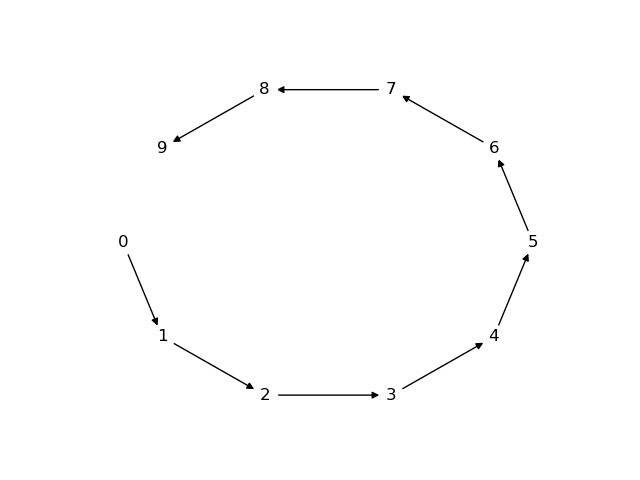
\includegraphics[width=0.4\textwidth]{images/instances_examples/too_easy.png}
    \caption{Example of an instance too easy to solve, the vertices are too tight to one another.}
\end{figure}

\begin{figure}[H]
    \centering
    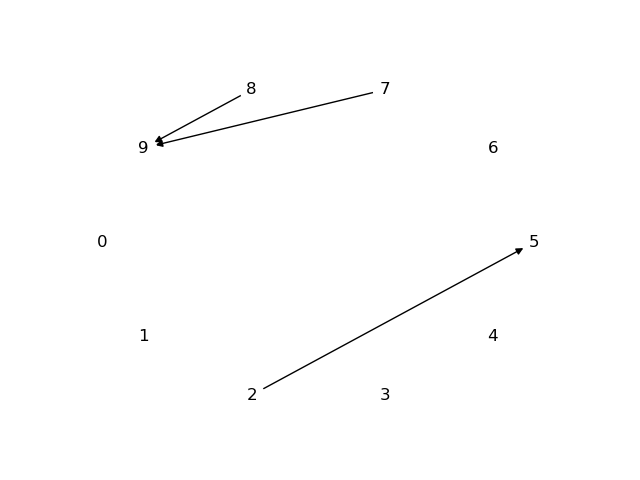
\includegraphics[width=0.4\textwidth]{images/instances_examples/too_difficult.png}
    \caption{Example of an instance too difficult to solve, the vertices are too loose from one another.}
\end{figure}

\begin{figure}[H]
    \centering
    \includegraphics[width=0.4\textwidth]{images/instances_examples/good.png}
    \caption{Example of a good instance, not too hard, not too easy. The vertices are somewhat tight to one another, but not too much.}
\end{figure}


\end{appendices}

\end{document}
